% \documentclass{beamer}
\documentclass[xcolor=dvipsnames]{beamer}
%% \usecolortheme[named=Blue]{structure}
\setbeamersize{text margin left=30mm, text margin right=30mm}
\useoutertheme{infolines}
%% \usetheme[height=7mm]{Rochester}
\usetheme{Pittsburgh}
\setbeamertemplate{items}[ball]
\setbeamertemplate{blocks}[rounded][shadow=true]
\setbeamertemplate{navigation symbols}{}

\usepackage[utf8x]{inputenc}
%% \usepackage{default}
\usepackage[english]{babel}
\usepackage{geometry}
%% \usepackage{fullpage}
\usepackage{amsmath, amsthm, amssymb}
\usepackage{listings}
\usepackage{pxfonts}
%% \usepackage{color}
%% \usepackage{graphicx}
%% \usepackage{natbib}
%% \usepackage{array}
%% \usepackage{booktabs}
%% \usepackage{tabu}
%% \usepackage[utf8]{inputenc}
%% \usepackage{fancyhdr}
%% \usepackage{float}
%% \usepackage{subfigure}
%% \usepackage{titlesec}

\setbeamertemplate{headline}{}
%% \setbeamertemplate{footline}[frame number]{}
\setbeamertemplate{navigation symbols}{}
%% \setbeamertemplate{footline}{}


\def\CCT{{C\nolinebreak[4]\hspace{-.05em}\raisebox{.4ex}{\tiny\bf ++}}}
\def\CC{{C\nolinebreak[4]\hspace{-.05em}\raisebox{.4ex}{\small\bf ++}}}


\definecolor{lstgray}{gray}{0.93}
\definecolor{strgray}{gray}{0.4}

\lstset{ %
  escapechar=@,
  language=C++,
  basicstyle=\footnotesize\ttfamily,
  %% basicstyle=\ttfamily,
  %% keywordstyle=\color{blue}\ttfamily,
  keywordstyle=\bfseries,
  stringstyle=\color{strgray}\ttfamily,
  commentstyle=\color{OliveGreen}\ttfamily,
  %% morecomment=[l][\color{red}]{\#},
  morecomment=[l][\color{blue}]{\#},
  backgroundcolor=\color{lstgray},
  %% keywordstyle=\color{red},
  frame=f,
  frameround=ffff,
  tabsize=2,
  breaklines=true,
  breakatwhitespace=false,
  showspaces=false,
  showstringspaces=false,
  xleftmargin=5pt,
  xrightmargin=5pt,
  morekeywords={in,out,ref,auto,inout,import,ushort,scope,exit,mixin,decltype,varid,sizeof,constexpr}
}

\def\redcolor{\color{red}}
\def\bluecolor{\color{blue}}
\def\blackcolor{\color{black}}
\def\graycolor{\color{gray}}
\def\greencolor{\color{OliveGreen}}


\def\sectionname{\translate{Section}}
\def\insertsectionnumber{\arabic{section}}
\setbeamertemplate{section page}
{
  \begin{centering}
    \begin{beamercolorbox}[sep=4pt,center]{part title}
      \usebeamerfont{section title}\insertsection\par
    \end{beamercolorbox}
  \end{centering}
}
\def\sectionpage{\usebeamertemplate*{section page}}


\AtBeginSection{\frame{\sectionpage}}


\title{Expression tree transforms}
\subtitle{For compile-time differentiation}
%% \author{\texorpdfstring{Author\newline\url{email@email.com}}{Dominic Jones}}
\author{Dominic Jones}
\date{\tiny{March 2018}}
%% \author{Author\\{\tiny email@email.com}}
\institute{\texttt{dominic.jones@gmx.co.uk}}


\begin{document}
\begin{frame}[plain]
  \titlepage
\end{frame}


\section{Differentiate a function \protect\textit{losslessly}}


\begin{frame}[fragile]{Parity preserving transform}
  \begin{columns}[T] % align columns
    \begin{column}{0.44\textwidth}
      {\color{gray}{write something like this \dots}}
      \begin{lstlisting}
fn(A const &a, B const &b,
   R &r)
{
  auto c0 = 7;
  auto c1 = 9;

  auto t0 = a * b;   // 1
  auto t1 = c0 + t0; // 2
  auto t2 = c1 + t0; // 3

  r  = t1 / t2;      // 4
}
  \end{lstlisting}
    \end{column}%
    \hfill%
    \begin{column}{0.56\textwidth}
      {\color{gray}{to implement something like this}}
        \begin{lstlisting}
fn(A const &a, B const &b,
   R &r)
{
  auto c0 = 7;
  auto c1 = 9;

  auto t0 = a * b;   // 1
  auto t1 = c0 + t0; // 2
  auto t2 = c1 + t0; // 3

  // somehow add this...
  t1.d += (1/t2)    * r.d; // 4'
  t2.d -= (t1/t2^2) * r.d; // 4'
  t0.d += t2.d;            // 3'
  t0.d += t1.d;            // 2'
  a.d  += b * t0.d;        // 1'
  b.d  += a * t0.d;        // 1'
}
  \end{lstlisting}
    \end{column}%
  \end{columns}
\end{frame}


\begin{frame}[fragile]{Observations}
  \begin{enumerate}
  \item Given a pure-functional algorithm, differentiate it \vspace{5mm}
  \item Implement the transpose of the chain of derivatives (the adjoint) \vspace{5mm}
  \item The required `extra' code is in the reversed sequence of the original and the data flow is reversed \vspace{5mm}
  \item Eager and lazy evaluation: ctor-dtor pairs? \vspace{5mm}
  \end{enumerate}
\end{frame}


\section{Two hurdles}


\begin{frame}[fragile]{Dealing with duplicate nodes}
Eager evaluation and capture by reference?
  \begin{columns}[T] % align columns
    \begin{column}{0.5\textwidth}
        \begin{lstlisting}
fn(A const &a, B const &b,
   R &r)
{
  auto c0 = 7;
  auto c1 = 9;

  auto @\aftergroup\bluecolor@t0@\aftergroup\blackcolor@ = a * b;
  auto t1 = c0 + @\aftergroup\bluecolor@t0@\aftergroup\blackcolor@; // l.b.
  auto t2 = c1 + @\aftergroup\bluecolor@t0@\aftergroup\blackcolor@; // r.b.

  r  = t1 / t2;      // root
}
  \end{lstlisting}
    \end{column}%
    \hfill%
    \begin{column}{0.5\textwidth}
\begin{figure}[H]
 \centering
 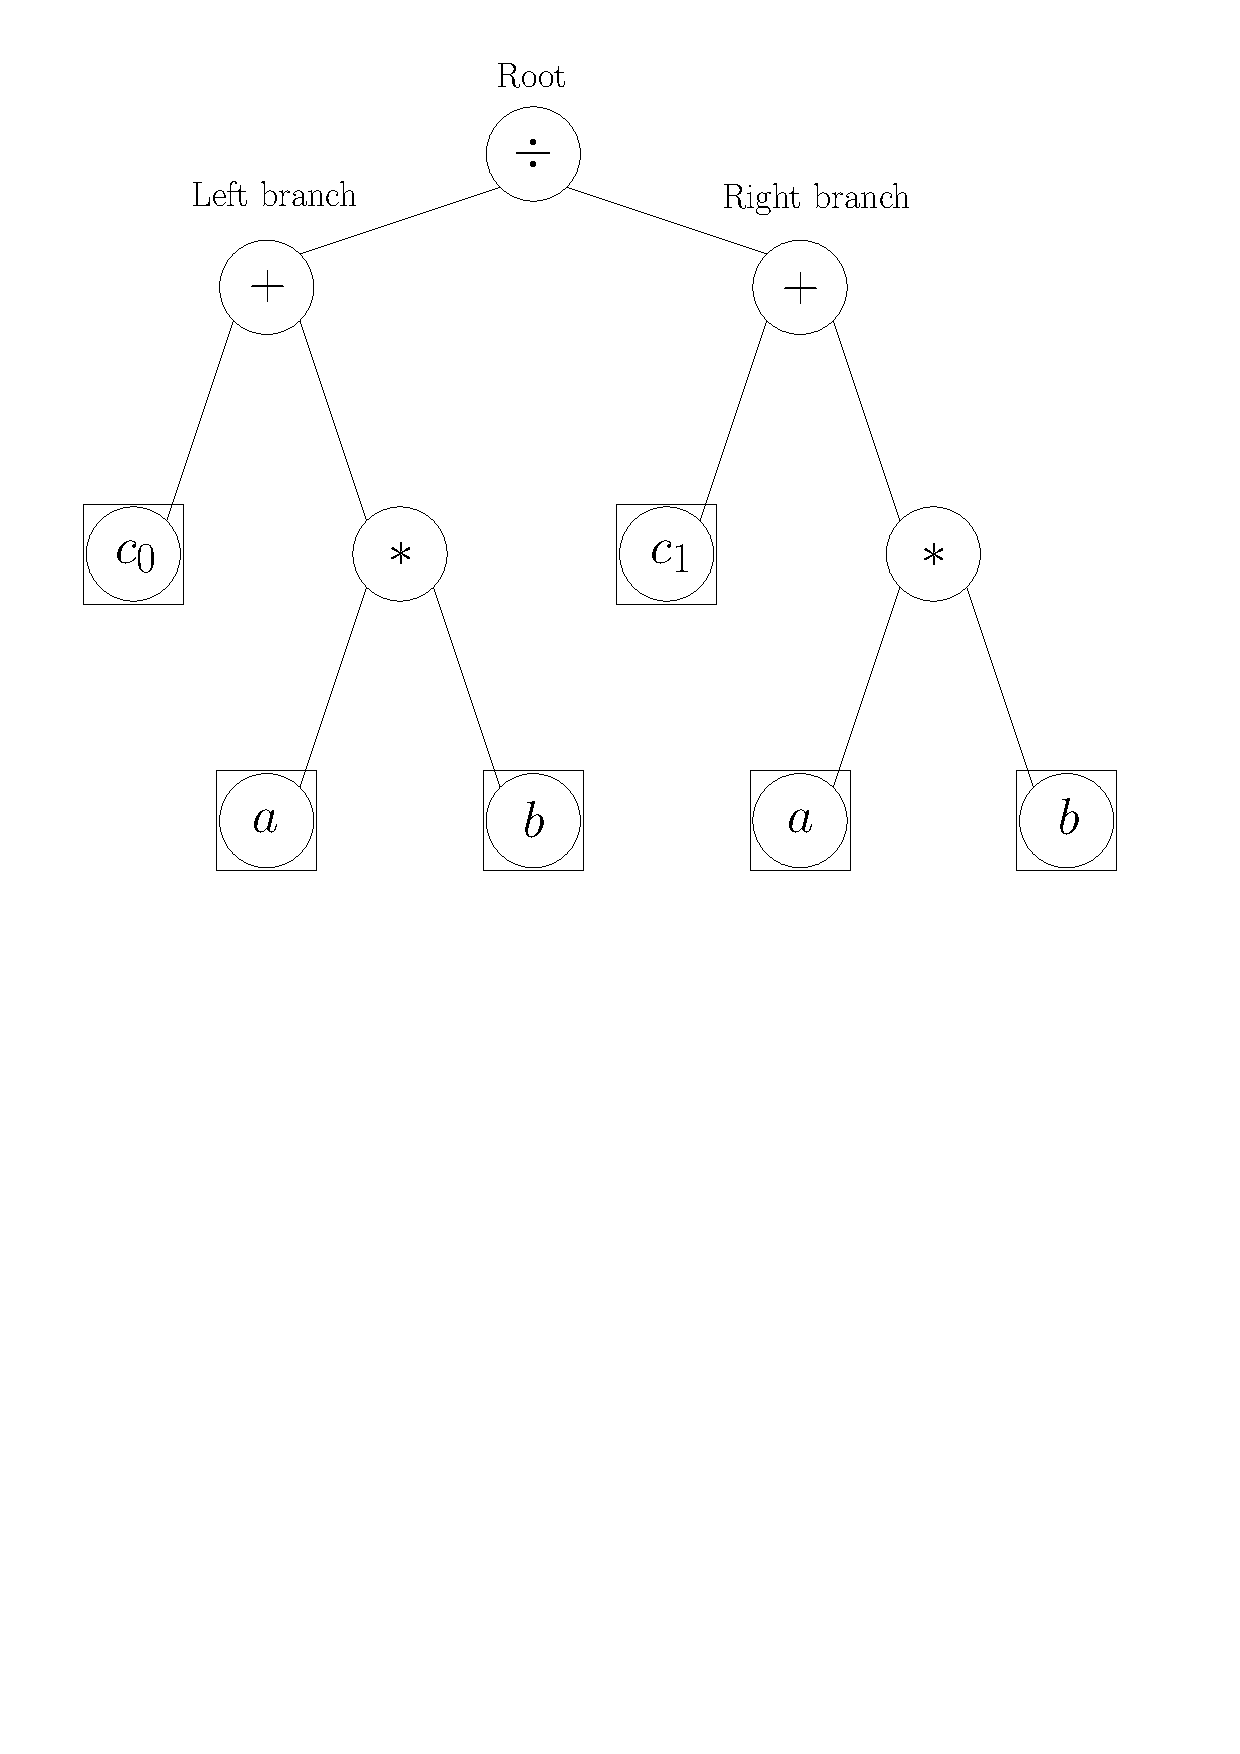
\includegraphics[width=0.99\textwidth]{fig_exprtree}
\end{figure}
    \end{column}%
  \end{columns}
\end{frame}


\begin{frame}[fragile]{Dealing with nested scoping}
The \emph{complete} tree, including {\color{red}\texttt{cm}}, is needed for the transform
  \begin{columns}[T] % align columns
    \begin{column}{0.44\textwidth}
        \begin{lstlisting}
fn(A const &a, B const &b,
   R &r)
{
  auto c0 = 7;
  auto c1 = 9;

  auto t0 = @\aftergroup\bluecolor@a * b@\aftergroup\blackcolor@;   // 1
  auto t1 = c0 + t0; // 2
  auto t2 = c1 + t0; // 3

  r  = t1 / t2;      // 4
}
  \end{lstlisting}
    \end{column}%
    \hfill%
    \begin{column}{0.56\textwidth}
      \begin{lstlisting}
@\aftergroup\bluecolor@mul@\aftergroup\blackcolor@(A const &a, B const &b)
{
  auto @\aftergroup\redcolor@cm@\aftergroup\blackcolor@ = 1; // lost on return!
  return @\aftergroup\redcolor@cm@\aftergroup\blackcolor@ * a * b;
}

fn(A const &a, B const &b, R &r)
{
  auto c0 = 7;
  auto c1 = 9;

  auto t0 = @\aftergroup\bluecolor@mul(a, b)@\aftergroup\blackcolor@;
  auto t1 = c0 + t0;
  auto t2 = c1 + t0;

  r  = t1 / t2;
}
  \end{lstlisting}
    \end{column}%
  \end{columns}
\end{frame}


\begin{frame}[fragile]{Dealing with nested scoping}
The \emph{complete} tree, including {\color{red}\texttt{cm}}, is needed for the transform
  \begin{columns}[T] % align columns
    \begin{column}{0.44\textwidth}
      \begin{lstlisting}
fn(A const &a, B const &b,
   R &r)
{
  auto c0 = 7;
  auto c1 = 9;
  auto @\aftergroup\redcolor@cm@\aftergroup\blackcolor@ = 1;
  auto t0 = @\aftergroup\redcolor@cm@\aftergroup\blackcolor@ * a * b;
  auto t1 = c0 + t0;
  auto t2 = c1 + t0;

  r  = t1 / t2;
}
  \end{lstlisting}
    \end{column}%
    \hfill%
    \begin{column}{0.56\textwidth}
        \begin{lstlisting}
fn(A const &a, B const &b,
   R &r)
{
  auto c0 = 3;
  auto c1 = 4;
  auto @\aftergroup\redcolor@cm@\aftergroup\blackcolor@ = 1;
  auto t0 = @\aftergroup\redcolor@cm@\aftergroup\blackcolor@ * a * b;
  auto t1 = c0 + t0;
  auto t2 = c1 + t0;

  // the transform...
  t1.d += (1/t2)    * r.d;
  t2.d -= (t1/t2^2) * r.d;
  t0.d += t2.d;
  t0.d += t1.d;
  a.d  += @\aftergroup\redcolor@cm@\aftergroup\blackcolor@ * b * t0.d;
  b.d  += @\aftergroup\redcolor@cm@\aftergroup\blackcolor@ * a * t0.d;
}
  \end{lstlisting}
    \end{column}%
  \end{columns}
\end{frame}


\begin{frame}[fragile]{State of affairs}
  \begin{enumerate}
  \item Eager evaluation avoids duplicate branch evaluation - but lazy evaluation will also be needed \vspace{5mm}
  \item `Capture by reference' to keep the tree small - but cannot work with nested scoping \vspace{5mm}
  \item `Capture by value' is too inefficient - the tree will get very large very quickly \vspace{5mm}
  \item A monolithic tree, supporting eager and lazy evaluation, of minimal size, and impartial to scoping is required \vspace{5mm}
  \end{enumerate}
  {\color{blue}Only capture terminals? - But how to know if they are already captured?} \vspace{5mm}
\end{frame}


\section{A `unique types' approach}


\begin{frame}[fragile]{Tagging terminals}
With all terminal types uniquely tagged, any duplicate branches can be identified
  \begin{columns}[T] % align columns
    \begin{column}{0.5\textwidth}
        \begin{lstlisting}
fn(A const &a, B const &b,
   R &r)
{
  auto c0 = @\aftergroup\bluecolor@UQ(@\aftergroup\blackcolor@7@\aftergroup\bluecolor@)@\aftergroup\blackcolor@; // unique
  auto c1 = @\aftergroup\bluecolor@UQ(@\aftergroup\blackcolor@9@\aftergroup\bluecolor@)@\aftergroup\blackcolor@; // unique

  auto t0 = a * b;
  auto t1 = c0 + t0;
  auto t2 = c1 + t0;

  r  = t1 / t2;
}
  \end{lstlisting}
    \end{column}%
    \hfill%
    \begin{column}{0.5\textwidth}
\begin{figure}[H]
 \centering
 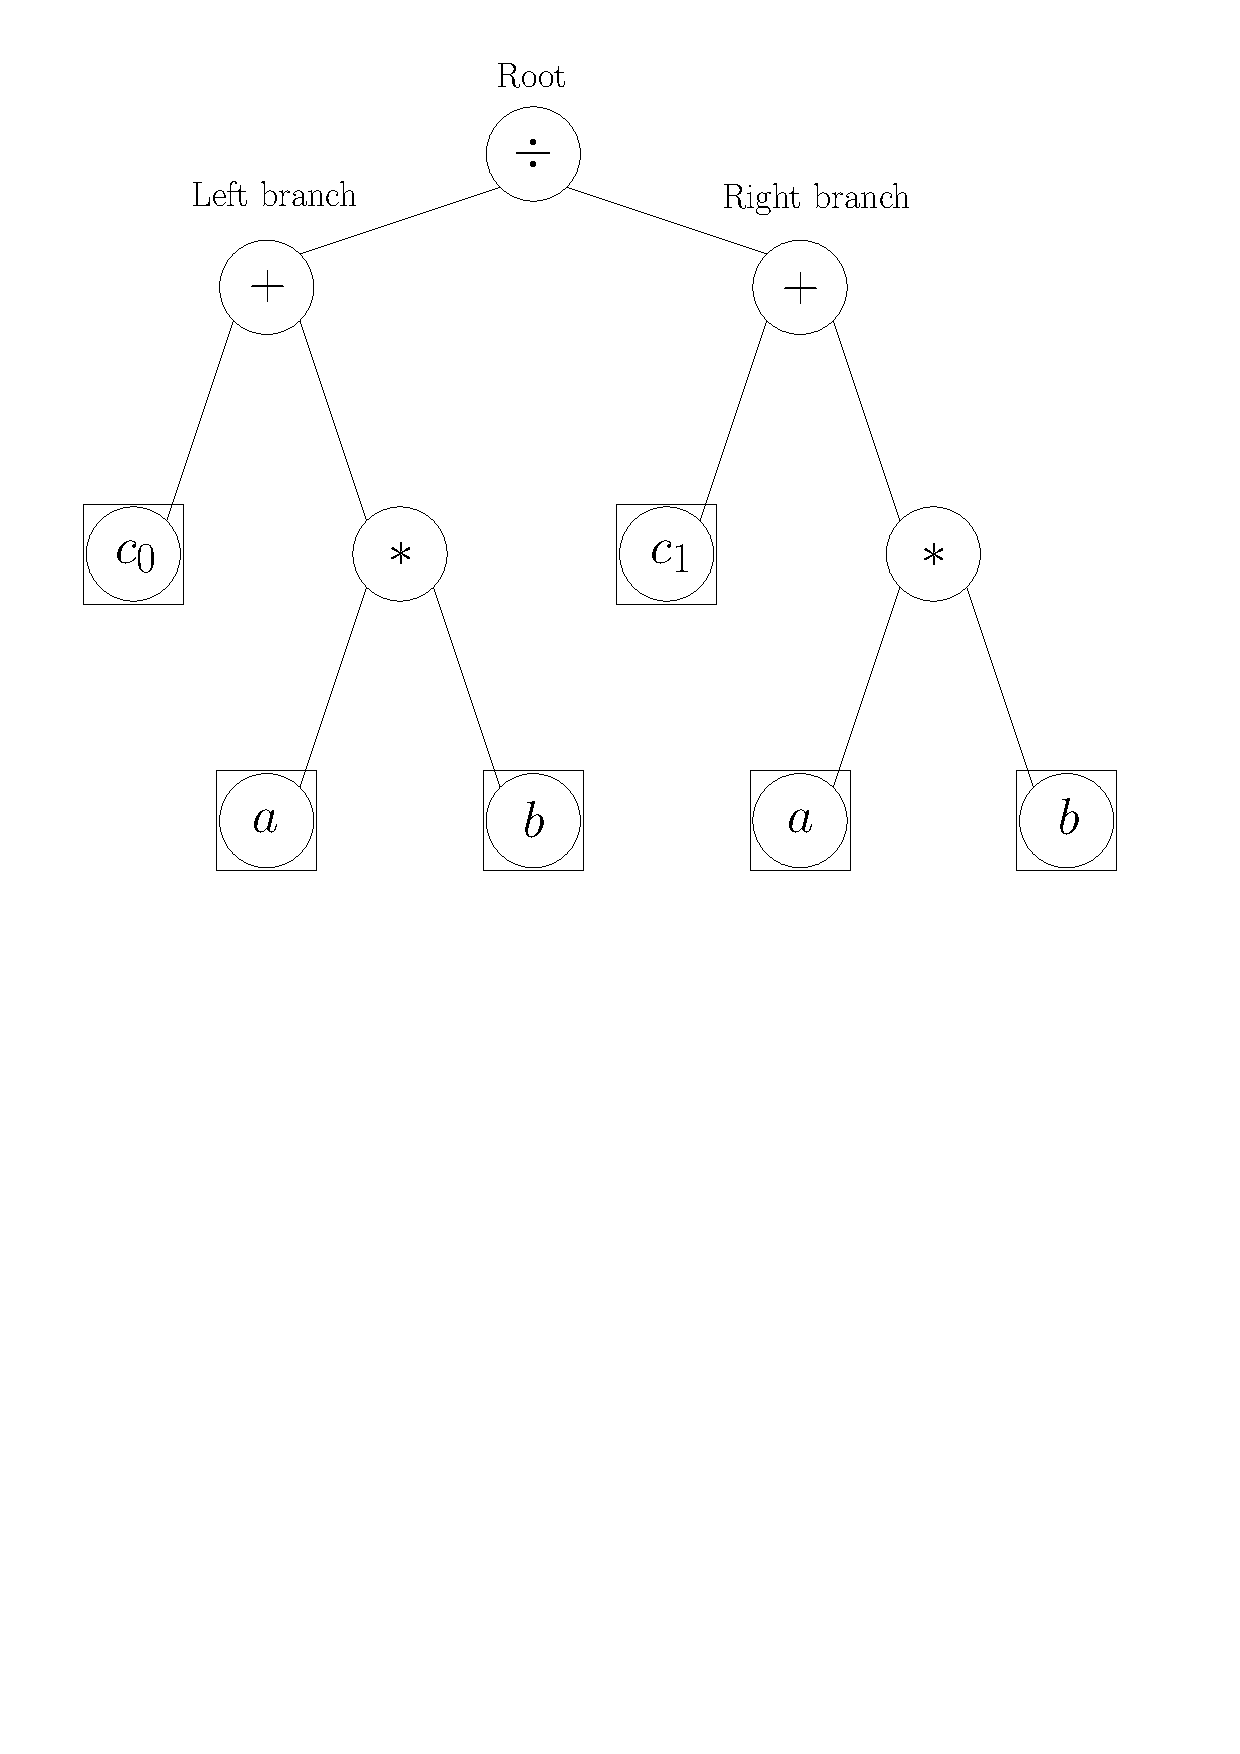
\includegraphics[width=0.99\textwidth]{fig_exprtree}
\end{figure}
    \end{column}%
  \end{columns}
\end{frame}


\begin{frame}[fragile]{Unique}
\begin{columns}[T] % align columns
    \begin{column}{0.44\textwidth}
  {\color{gray}Ugly, but works}
        \begin{lstlisting}
template<std::size_t ID,
         typename T>
struct Unique
{
  T value;
};
@\aftergroup\bluecolor@
#define UQ(v)          \
Unique<__COUNTER__,    \
       decltype(v)>{v}
@\aftergroup\blackcolor@
  \end{lstlisting}
    \end{column}%
    \hfill%
    \begin{column}{0.56\textwidth}
      {\color{gray}Interesting, yet useless}
\begin{lstlisting}
template<typename T, typename U>
auto constexpr
cmp(T const &t, U const &u)
{
  // Not possible!
  // auto constexpr ta = &t;
  // auto constexpr ua = &u;
  // return ta == ua;
  return @\aftergroup\bluecolor@&t == &u@\aftergroup\blackcolor@;
}

{
  auto c0 = 7;
  auto c1 = 9;

  static_assert(cmp(c0, c0));
  static_assert(!cmp(c0, c1));
}
\end{lstlisting}
    \end{column}%
  \end{columns}
\end{frame}


\section{Building the components}


\begin{frame}[fragile]{Bookkeeping}
  \begin{columns}[T] % align columns
    \begin{column}{0.5\textwidth}
      Types and data to percolate up the tree: \vspace{5mm}
      \begin{enumerate}
      \item Hierarchically grouped node types\newline ({\color{blue}\texttt{Binary<Mul, A, B>}}, etc) \vspace{5mm}
      \item List of constant values\newline ({\color{blue}\texttt{c0}} and {\color{blue}\texttt{c1}}) \vspace{5mm}
      \item List of argument addresses\newline ({\color{blue}\texttt{a}} and {\color{blue}\texttt{b}}) \vspace{5mm}
      \end{enumerate}
    \end{column}%
    \hfill%
    \begin{column}{0.5\textwidth}
\begin{figure}[H]
 \centering
 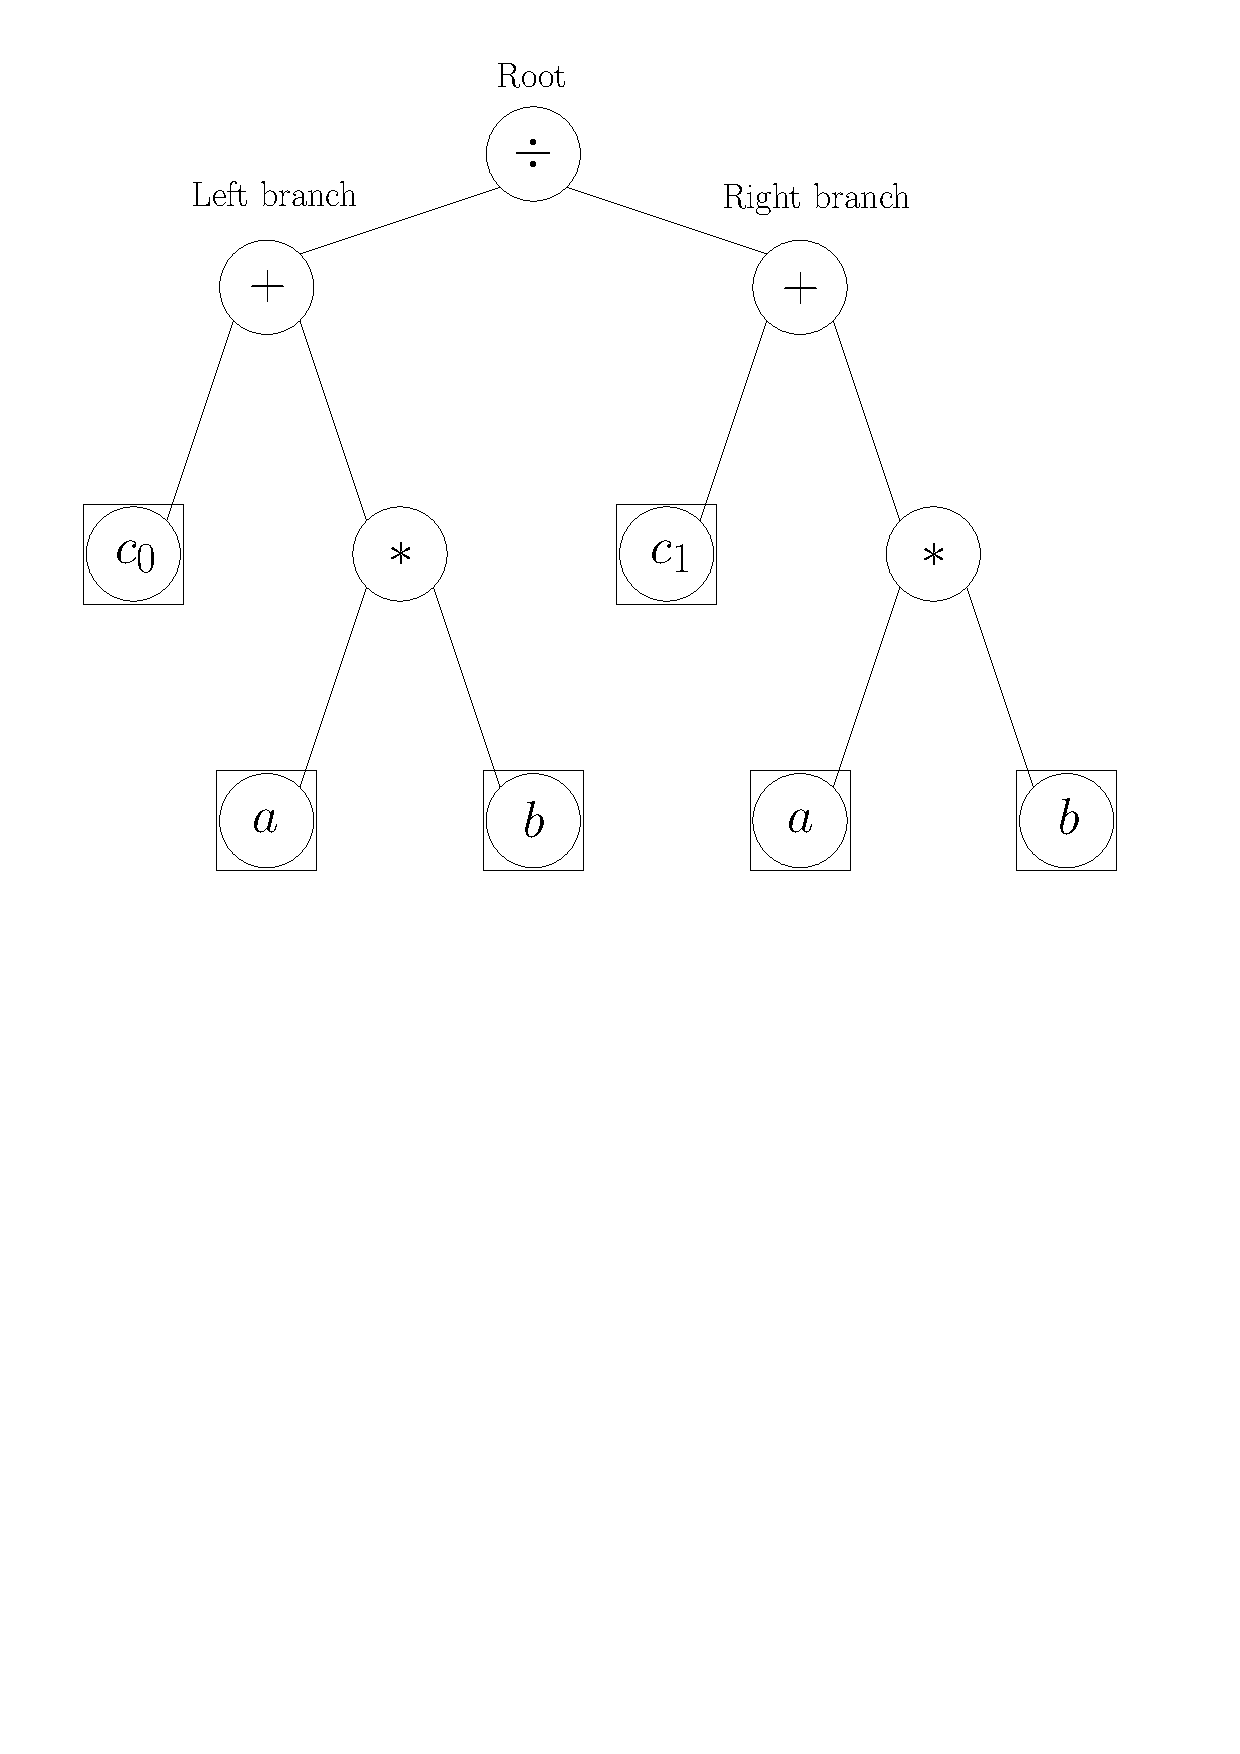
\includegraphics[width=0.99\textwidth]{fig_exprtree}
\end{figure}
    \end{column}%
  \end{columns}
\end{frame}


\begin{frame}[fragile]{Hierarchically grouped node types}
In the {\color{blue}root} node:
\begin{lstlisting}
// Pad left and right branches to equal depths
\end{lstlisting}
\begin{lstlisting}
// Merge left and right branches:
  {{A, B, @\aftergroup\redcolor@A, B@\aftergroup\blackcolor@},
   {Binary<Mul, A, B>, @\aftergroup\redcolor@Binary<Mul, A, B>@\aftergroup\blackcolor@},
   {Binary<Add, C0, ...>, @\aftergroup\redcolor@Binary<Add, C1, ...>@\aftergroup\blackcolor@}}
\end{lstlisting}
\begin{lstlisting}
// Prune duplicates:
  {{A, B},
   {Binary<Mul, A, B>},
   {Binary<Add, C0, ...>, Binary<Add, C1, ...>}}
\end{lstlisting}
\begin{lstlisting}
// Augment with self:
  {{A, B},
   {Binary<Mul, A, B>},
   {Binary<Add, C0, ...>, Binary<Add, C1, ...>},
   @\aftergroup\bluecolor@{Binary<Div, ...C0..., ...C1...>}@\aftergroup\blackcolor@}
\end{lstlisting}
\end{frame}


\begin{frame}[fragile]{Hierarchically grouped node types}
  \begin{enumerate}
  \item Prune duplicate branches eagerly \vspace{5mm}
  \item TMP operations exclusively on types \vspace{5mm}
  \item Relatively low compile-time overhead \vspace{5mm}
  \item Moderately involved: \texttt{resize}, \texttt{unique\_merge}, \texttt{append} \vspace{5mm}
  \item Using the Brigand library \vspace{5mm}
  \end{enumerate}
\end{frame}


\begin{frame}[fragile]{List of constant values}
In the {\color{blue}root} node:
\begin{lstlisting}
// Identify the longer list:
  LLC = get_longer<L::LC, R::LC>   @\aftergroup\bluecolor@i.e. {C0}@\aftergroup\blackcolor@
  SLC = get_shorter<L::LC, R::LC>  @\aftergroup\bluecolor@i.e. {C1}@\aftergroup\blackcolor@
\end{lstlisting}
\begin{lstlisting}
// Convert lists to sets:
  LSC = brigand::as_set<LLC>
  SSC = brigand::as_set<SLC>
\end{lstlisting}
\begin{lstlisting}
// Merge sets and convert to tuple:
  TC = rename<merge_sets<LSC, SSC>, tuple>
  TC const tc;  @\aftergroup\bluecolor@i.e. tuple of constants@\aftergroup\blackcolor@
\end{lstlisting}
\begin{lstlisting}
// Difference between tuple and longer list:
  S = drop<TC, size<LLC> >  @\aftergroup\bluecolor@i.e. {C1}@\aftergroup\blackcolor@
\end{lstlisting}
\begin{lstlisting}
// Construct `tc' member: (biggest source of inefficiency!)
  tc{tuple_cat(get_longer(l.tc, r.tc),
               @\aftergroup\bluecolor@select(@\aftergroup\blackcolor@S{}, get_shorter(l.tc, r.tc)@\aftergroup\bluecolor@)@\aftergroup\blackcolor@)}
\end{lstlisting}
\end{frame}


\begin{frame}[fragile]{List of constant values}
  \begin{enumerate}
  \item Heavy work done on smaller data \vspace{5mm}
  \item TMP operations on types and data \vspace{5mm}
  \item Significant compile-time overhead due to data operations \vspace{5mm}
  \item Bridging the type-value divide with {\color{blue}\texttt{select(S, L)}}\newline \textbf{\emph{This should be optimised}} \vspace{5mm}
  \end{enumerate}
\end{frame}



\begin{frame}[fragile]{\texttt{select}}
  \begin{columns}[T]
    \begin{column}{0.62\textwidth}
      \begin{lstlisting}[basicstyle=\scriptsize\ttfamily]
// a naive approach...

template<
  template<class...> class S, class... SS,
  template<class...> class L, class... LL>
S<SS...> select_impl(S<SS...>, L<LL...> l)
{
  // std::get will not work
  return S<SS...>{alt::get<SS>(l)...};
}

template<class S, class L>
S select(S s, L l)
{
  return select_impl(s, l);
}

using S = std::tuple<bool,float>;
using L = std::tuple<char,bool,int,float>;

select(S{}, L{'0', true, 2, 3.0});
      \end{lstlisting}
    \end{column}
    \hfill
    \begin{column}{0.4\textwidth}
      \vspace{5mm}
      \emph{Possible optimisation}:\newline Given that types are unique and ordered, if any \texttt{S} is found in \texttt{L}, \texttt{L} can be left-cropped\newline
      %% \vspace{5mm}

      Better to avoid \texttt{std::get<T>} altogether
    \end{column}
  \end{columns}
\end{frame}



\section{Doing something with all of it}


\begin{frame}[fragile]{Assigning to the result}
  \begin{columns}[T] % align columns
    \begin{column}{0.56\textwidth}
\begin{lstlisting}
template<typename T>
struct Result
{
  template<typename Expr>
  void operator=(Expr &expr)
  {
    // depth-grouped node list
    using LN = Expr::LN;

    // list of constants
    using LC = Expr::LC;
    auto &tc = expr.tc;

    // list of argument ptrs
    using LA = Expr::LA;
    auto &ta = expr.ta;

    // Now what?
  }
};
\end{lstlisting}
    \end{column}%
    \hfill%
    \begin{column}{0.44\textwidth}
      \vspace{5mm}
      Now construct the index arrays to access data: \vspace{5mm}
      \begin{enumerate}
      \item build left and right node lists \vspace{5mm}
      \item build offset arrays for left and right node lists \vspace{5mm}
      \item build offset array for constants, in order to construct its {\color{blue}dual} \vspace{5mm}
      \end{enumerate}
    \end{column}%
  \end{columns}
\end{frame}


\begin{frame}[fragile]{Converting to offsets}
%%
\begin{lstlisting}
// Flatten the node list (6 elements)
  LN =  {A, B,
         Binary<Mul, A, B>,
         Binary<Add, C0, ...>, Binary<Add, C1, ...>,
         Binary<Div, ...C0..., ...C1...>}
\end{lstlisting}
%%
\begin{lstlisting}
// Offsets of left child nodes (`6' = null marker)
  INL = {6, 6, 0, 6, 6, 3}

// Offsets of right child nodes
  INR = {6, 6, 1, 2, 2, 4}
\end{lstlisting}
%%
\begin{lstlisting}
// With the list of constants...
  LC =  {Binary<Add, C0, ...>, Binary<Add, C1, ...>}

// generate node list offsets...
  IC =  {3, 4}

// then construct its `dual' (`2' = null marker)
  DC =  {2, 2, 2, 0, 1, 2}
\end{lstlisting}
%%
\begin{lstlisting}
\end{lstlisting}
\end{frame}


\begin{frame}[fragile]{`Eager and lazy' evaluation}
Inside the result assignment operator (pseudocode):
\begin{lstlisting}
// Initialise array/tuple data (6 elements)
  array<double, 6> v = 0;

// set input from tuple of argument ptrs
  for (i = 0; i != ta.size(); ++i)
    v[i] = *ta[i];
\end{lstlisting}
%%
\begin{lstlisting}
// evaluate operators
  for (N: LN)
    I = offset<N, LN>;
    N::evaluate<I>(v, tc, INL{}, INR{}, DC{})
\end{lstlisting}
%%
\begin{lstlisting}
// extract result from `root' node
  this.r = v[v.size()-1];
\end{lstlisting}
%%
\begin{lstlisting}
  @\aftergroup\bluecolor@... then the reverse order to differentiate@\aftergroup\blackcolor@
\end{lstlisting}
\end{frame}


\begin{frame}[fragile]{Results}
\textbf{Case 1}: nodes: 82, depth: 37, inputs: 2, constants: 12
\begin{table}
\begin{tabular}{l | c | c | c | c }
Version & compilation & original & auto diff & manual diff \\
\hline \hline
\texttt{alt::tuple} & 2.2s & 1x & 1.25x & 1.48x \\
\texttt{std::tuple} & 4.5s & 1x & 1.25x & 1.48x \\
\end{tabular}
\end{table}
\vspace{10mm}
\textbf{Case 2}: nodes: 331, depth: 25, inputs: 5, constants: 103
\begin{table}
\begin{tabular}{l | c | c | c | c }
Version & compilation & original & auto diff & manual diff \\
\hline \hline
\texttt{alt::tuple} & 59s & 1x & 5.7x & 1.9x \\
\texttt{std::tuple} & 27m & 1x & 4.7x & 1.9x \\
\end{tabular}
\end{table}
\end{frame}


\begin{frame}[fragile]{Conclusion}
  \begin{enumerate}
  \item Manipulation the tree is obtained at immense effort \vspace{5mm}
  \item Works in the range of exceptionally well (better than hand coded) to acceptably well (better than alternatives) \vspace{5mm}
  \item Compile-time features of the language are too limited to use this approach neatly \vspace{5mm}
  \item Inlining gives up too readily: \verb$__attribute__((always_inline))$ used ubiquitously \vspace{5mm}
  \item Not obvious what is going on with \verb$std::tuple$ \vspace{5mm}
  \end{enumerate}
\end{frame}


\section{Footnotes}


\begin{frame}[fragile]{Learning the ropes}
  \begin{enumerate}
  \item Peter Dimov's ``Simple C++ metaprogramming'' articles \vspace{5mm}
  \item Time the compilation for large data sets \vspace{5mm}
  \item An optimised \texttt{reverse} function is critical \vspace{5mm}
  \item Brigand library is an excellent resource \vspace{5mm}
  \end{enumerate}
\end{frame}


\begin{frame}[fragile]{Reflect compile-time literals}
  \begin{columns}[T] % align columns
    \begin{column}{0.52\textwidth}
\begin{center}Possible\end{center}
  \begin{lstlisting}
// Boost Hana extension...
#ifdef CONFIG_ENABLE_STRING_UDL



auto constexpr x =
  hana::string_c<'a','b','c'>;

auto constexpr y = "abc"_s;

CONSTANT_CHECK(x == y);
  \end{lstlisting}
    \end{column}%
    \hfill%
    \begin{column}{0.55\textwidth}
\begin{center}Desirable\end{center}
      \begin{lstlisting}
template<auto v>
struct Literal {
auto constexpr static value = v;
};

auto constexpr x =
  @\aftergroup\redcolor@Literal<4.2>@\aftergroup\blackcolor@;

auto constexpr y = @\aftergroup\redcolor@4.2_f@\aftergroup\blackcolor@;

static_assert(
  std::is_same_v<decltype(x),
                 decltype(y)>);
 \end{lstlisting}
    \end{column}%
  \end{columns}
\end{frame}


\begin{frame}[fragile]{Reflect compile-time location}
  \begin{columns}[T] % align columns
    \begin{column}{0.47\textwidth}
\begin{center}Possible\end{center}
  \begin{lstlisting}
@\aftergroup\graycolor@ 123456789 123456789 12345
         10        20
1
2  // main.cpp
3
4@\aftergroup\blackcolor@  decltype(x)* y = &x;@\aftergroup\graycolor@
5
@\aftergroup\bluecolor@   reflect          reflect
   type             address@\aftergroup\graycolor@
  \end{lstlisting}
    \end{column}%
    \hfill%
    \begin{column}{0.53\textwidth}
\begin{center}Desirable\end{center}
 \begin{lstlisting}
@\aftergroup\graycolor@ 123456789 123456789 12345
         10        20
1
2  // main.cpp
3
4@\aftergroup\blackcolor@  auto constexpr y = &x;@\aftergroup\graycolor@
5
@\aftergroup\redcolor@                      reflect
                      location@\aftergroup\graycolor@


@\aftergroup\redcolor@y = hash(row, column, filename)@\aftergroup\graycolor@
@\aftergroup\redcolor@  = hash(4, 23, "main.cpp")@\aftergroup\graycolor@

 \end{lstlisting}
    \end{column}%
  \end{columns}
\end{frame}


\begin{frame}[fragile]{Function signature pattern}
\begin{lstlisting}
struct @\aftergroup\bluecolor@_1@\aftergroup\blackcolor@;  struct @\aftergroup\bluecolor@_2@\aftergroup\blackcolor@;
template<template<class...> class, class...> struct bind;

// Apply a function taking two args to a list...
template<class L, class P> struct apply;

template<template<class...> class L, class T, class... Ts,
         template<class...> class F>
struct apply<L<T, Ts...>, bind<F, @\aftergroup\bluecolor@_1@\aftergroup\blackcolor@, @\aftergroup\bluecolor@_2@\aftergroup\blackcolor@> >
{
  using type = L<F<T, Ts>...>;
};

// A function taking two args...
template<class T, class U>
using cmp = bool_t<(sizeof(T) > sizeof(U))>;

// evaluate `cmp' over a list
using L = list<int, bool, char, double>;
using R = apply<L, bind<cmp, @\aftergroup\bluecolor@_1@\aftergroup\blackcolor@, @\aftergroup\bluecolor@_2@\aftergroup\blackcolor@> >::type;
\end{lstlisting}
\end{frame}


\end{document}
